\documentclass[a4paper, 12pt]{scrartcl}

\usepackage[utf8]{inputenc}
\usepackage[ngerman]{babel}

\usepackage{mathptmx}
\renewcommand{\familydefault}{\sfdefault}

% Settings for page geometry
\usepackage[left=2.5cm, right=2.5cm, top=2.5cm, bottom=2.5cm]{geometry}
\usepackage[onehalfspacing]{setspace}

% ETC Packages
\usepackage{amsmath}
\usepackage{amssymb}
\usepackage{graphicx}
\usepackage{xcolor}
\usepackage{floatflt,epsfig}
\usepackage{scrlayer-scrpage}
\usepackage{hyperref}
\usepackage{float}
\usepackage{sectsty}

\usepackage{xcolor}
\usepackage{floatflt,epsfig}
\usepackage[framemethod=tikz]{mdframed}
% \usepackage[fleqn]{amsmath}
\usepackage{listings}
\usepackage{color}
%\usepackage{minted}

\mdfsetup{
    skipabove=\topskip ,
    skipbelow=\topskip ,
    innertopmargin=-0.2cm,
    innerbottommargin=-0.2cm,
    innerleftmargin=0cm
}

\definecolor{dkgreen}{rgb}{0,0.6,0} % comment style
\definecolor{gray}{rgb}{0.5,0.5,0.5}
\definecolor{mauve}{rgb}{0.58,0,0.82} 
\definecolor{BBS}{RGB}{0,169,164} % Teal color of BBS logo
\definecolor{ssh}{RGB}{22,198,12} % bash connection / user
\definecolor{path}{RGB}{59,120,184} % Bash current working directory
\definecolor{bbg}{RGB}{50,50,50} % Bash Background
\definecolor{cfg}{RGB}{58,150,221} % Bash Background

\lstset{ % defining an environment for bash code
    escapeinside={<@}{@>},
    aboveskip=3mm,
    belowskip=3mm,
    showstringspaces=false,
    columns=flexible,
    basicstyle={\small\ttfamily\color{white}},
    numbers=none,
    numberstyle=\tiny\color{white},
    commentstyle=\color{dkgreen},
    stringstyle=\color{blue},
    breaklines=true,
    breakatwhitespace=true,
    tabsize=3,
    morekeywords={
        sudo, apt, git, ufw
    }
}

% Define colors for headings of different parts of the documentation
\sectionfont{\color{BBS}}
\subsectionfont{\color{BBS}}
\subsubsectionfont{\color{BBS}}

\begin{document}
% \begin{spacing}{1.3}
\thispagestyle{empty}
\ihead{
    \begin{footnotesize}
        Deployment einer Rest API
    \end{footnotesize}
}
\chead{
    \begin{footnotesize}
        Lernfeld 9: Netzwerke und Dienste bereitstellen
    \end{footnotesize}
}
\ohead{
    \begin{footnotesize}
        Gerrit Koppe
    \end{footnotesize}
}
\vspace{0.2\textheight}
\begin{center}
    \begin{figure}[H]
        \begin{minipage}{0.3\textwidth}
            
\includegraphics[scale=0.6]{Bilder/BBS}
        \end{minipage}
        \hspace{0.48\textwidth}
        \begin{minipage}{0.3\textwidth}
            
\includegraphics[scale=0.6]{Bilder/sievers.png}
        \end{minipage}
    \end{figure}
    \vspace{1cm}
    \begin{Huge}
        \textcolor{BBS}{\textbf{Dokumentation Deployment einer Rest API}}
    \end{Huge}
    \\
    \vspace{0.1\textheight}
    \begin{Large}
        Autor: Gerrit Koppe
    \end{Large}
    \\
    \vspace{0.5cm}
    \begin{Large}
        Ausbildungsberuf: Fachinformatiker für Anwendungsentwicklung
    \end{Large}
    \\
    \vspace{0.5cm}
    \begin{Large}
        Klasse: IFA12
    \end{Large}
    \\
    \vspace{0.5cm}
    \begin{Large}
        Lernfeld 9: Netzwerke und Dienste bereitstellen
    \end{Large}
    \\
    \vspace{0.5cm}
    \begin{Large}
        \today
    \end{Large}
\end{center}
\newpage
\thispagestyle{empty}
\begin{Large}
    \begin{flushleft}
        \textbf{\textcolor{BBS}{Anmerkungen}}
    \end{flushleft}
\end{Large}
Aus Gründen der Leserlichkeit wird in dieser Dokumentation das Wort \glqq Server\grqq{} verwendet, wann immer vom Raspberry Pi die Rede ist.
\\
Manche der hier in der Dokumentation beschriebenen Befehle mussten bei der Ausführung bestätigt werden. Die Bestätigung wird nicht explizit
erwähnt.
\\
Wann immer in einer Terminal Abbildung \glqq\lstinline[basicstyle={\small\ttfamily\color{black}}]|#...|\grqq{} steht, zeigt dies an, dass die Datei, welche jeweils bearbeitet wurde,
weitere Zeilen hat, welche aber nicht relevant für den jeweils aktuellen Arbeitsschritt sind und dementsprechend ausgelassen wurden. Es kann außerdem anzeigen, dass
die Kommandozeile nach Ausführung eines Befehls noch weitere Informationen anzeigt, diese allerdings ebenfalls ausgelassen wurden.
\\
Aus technischen Gründen, wurde ab dem Kapitel \glqq Einrichtung Webserver\grqq{} nicht mehr auf einem Raspberry Pi, sondern auf einem Ubuntu Server 22.04 gearbeitet. Es ist möglich,
dass manche Kommandos sich zu denen, die auf einem Raspberry Pi ausgeführt werden würden, unterscheiden.
\\
Da die in dieser Dokumentation beschriebene Installation auf Servern durchgeführt wurde, die nur aus bestimmten Netzwerken erreichbar sind und die Server nach Abgabe der Dokumentation
heruntergefahren werden, wurde darauf verzichtet, IP-Adressen, Benutzer und Passwörter unkenntlich zu machen, da dadurch die Leserlichkeit hätte beeinträchtigt werden können.


\newpage
\thispagestyle{empty}
\tableofcontents
\newpage
\clearpage
\pagenumbering{arabic}


\section{Einleitung}
In dieser Dokumentation wird die Konfiguration eines Raspberry Pi\footnote{Fortan \glqq Server\grqq} als Host einer Rest API, sowie das Deployment besagter Rest API beschrieben.
\\
Es wird zunächst auf allgemeine Vorbereitungen eingegangen. Anschließend wird beschrieben, wie die User und das Netzwerk, sowie die Firewall des Servers konfiguriert werden müssen.
Abschließend wird die Installation des Webservers, sowie das Deployment der Rest API und der Nextcloud Lösung als Docker Container auf dem Server beschrieben.
\\
Sämtliche Arbeitsschritte sind durch die Terminal Befehle dokumentiert, die während der Umsetzung ausgeführt wurden.



\section{Vorbereitungen}
Bevor die Aufgabe selbst begonnen werden konnte, musste zunächst eine SD Karte mit dem Raspbian OS beschrieben werden. Diese Aufgabe wurde von Herrn Wichmann durchgeführt.
\\
Nachdem das Raspbian OS erfolgreich auf der SD Karte installiert wurde und die SD-Karte im Server verbaut wurde, musste der Server per Ethernet Kabel an ein Netzwerk
angeschlossen werden, zu dem der Umsetzende Zugriff hatte.
\\
Schlussendlich wurde eine Verbindung zum Server per SSH aufgebaut. Da noch keine Änderungen am Betriebssystem vorgenommen wurden, wurde die Verbindung mit dem Benutzer
\glqq pi\grqq{} und dem Passwort \grqq raspberry\grqq{} aufgebaut:
\begin{figure}[H]
    \begin{mdframed}[backgroundcolor=bbg]
        \begin{lstlisting}
        C:\Users\gkoppe>ssh pi@192.168.24.113
        pi@192.168.24.113's password:
        \end{lstlisting}
    \end{mdframed}
    \label{lst:user_72}
    % \caption{benutzer72 anlegen}
\end{figure}



\section{Konfiguration der User}\label{ch:user}
% Benötigte User und warum
% TODO Begründung anpassen.
Nachdem das Betriebssystem des Servers installiert, der Server in das Netzwerk eingebunden und überprüft wurde, ob eine SSH Verbindung zum Server möglich ist, wurden zwei neue User angelegt, um den Server
abzusichern, da der User \glqq Pi\grqq{} der Standarduser des Betriebssystems und somit allgemein bekannt ist.
\\
Es wurden insgesamt zwei neue User angelegt. Ein User \glqq benutzer72\grqq{} mit grundlegenden Nutzungsrechten und ein Benutzer \glqq fernzugriff\grqq{} mit administrativen Rechten. Des Weiteren kann der
Benutzer \glqq fernzugriff\grqq{} verwendet werden, um eine SSH-Verbindung zum Server aufzubauen.
\subsection{Anlage neuer Benutzer}\label{ch:user_add}
Zunächst wurde der user \glqq benutzer72\grqq{} mit folgenden Befehlen angelegt:
\begin{figure}[H]
    \begin{mdframed}[backgroundcolor=bbg]
        \begin{lstlisting}
        <@\textcolor{ssh}{pi@raspberry}@>:<@\textcolor{path}{$\sim$ \$}@> sudo useradd -m benutzer72
        <@\textcolor{ssh}{pi@raspberry}@>:<@\textcolor{path}{$\sim$ \$}@> sudo passwd benutzer72
        New password:
        Retype new password:
        passwd: password updated successfully
        \end{lstlisting}
    \end{mdframed}
    \label{lst:user_72}
    % \caption{benutzer72 anlegen}
\end{figure}
Der Befehl \lstinline[basicstyle={\small\ttfamily\color{black}}]|useradd| dient dazu, den neuen Benutzer anzulegen. Mit dem flag \lstinline[basicstyle={\small\ttfamily\color{black}}]|-m| wird außerdem
automatisch ein Home-Verzeichnis für den neuen Benutzer erzeugt. Des Weiteren wurde dem neuen Benutzer mittels des \lstinline[basicstyle={\small\ttfamily\color{black}}]|passwd| Befehls ein neues Passwort
zugewiesen.
\\
Nachdem der Benutzer benutzer72 konfiguriert wurde, wurde ein neuer administrativer Nutzer \glqq fernzugriff\grqq{} angelegt. Die Vorgehensweise war hier zunächst identisch zu der der Neuanlage von
benutzer72:
\begin{figure}[H]
    \begin{mdframed}[backgroundcolor=bbg]
        \begin{lstlisting}
        <@\textcolor{ssh}{pi@raspberry}@>:<@\textcolor{path}{$\sim$ \$}@> sudo useradd -m fernzugriff
        <@\textcolor{ssh}{pi@raspberry}@>:<@\textcolor{path}{$\sim$ \$}@> sudo passwd fernzugriff
        New password:
        Retype new password:
        passwd: password updated successfully
        \end{lstlisting}
    \end{mdframed}
    \label{lst:user_fernzugriff}
    % \caption{fernzugriff anlegen}
\end{figure}

\subsection{Konfiguration des administrativen Benutzers}\label{ch:user_admincfg}
Da der Benutzer \glqq fernzugriff\grqq{} administrative Rechte auf dem Server erhalten sollte, wurde er anschließend in die Gruppe \glqq sudo\grqq{} aufgenommen:
\begin{figure}[H]
    \begin{mdframed}[backgroundcolor=bbg]
        \begin{lstlisting}
        <@\textcolor{ssh}{pi@raspberry}@>:<@\textcolor{path}{$\sim$ \$}@> sudo usermod -aG sudo fernzugriff
        \end{lstlisting}
    \end{mdframed}
    \label{lst:usermod_fernzugriff}
    % \caption{fernzugriff anlegen}
\end{figure}
Hier dient der Befehl \lstinline[basicstyle={\small\ttfamily\color{black}}]|usermod| allgemein dazu, einen User zu modifizieren. Der Flag \lstinline[basicstyle={\small\ttfamily\color{black}}]|-aG| gibt an,
dass der User einer Gruppe hinzugefügt werden soll, welche wiederum direkt hinter dem Flag definiert ist (in diesem Fall \glqq sudo\grqq).
\\
Abschließend wurde dem Benutzer \glqq fernzugriff\grqq{} noch das Recht gewährt, sich per SSH mit dem Server zu verbinden. Dafür wurde die Einstellung \lstinline[basicstyle={\small\ttfamily\color{black}}]|AllowUsers|
in der Datei \lstinline[basicstyle={\small\ttfamily\color{black}}]|/etc/ssh/sshd_config|:

\begin{figure}[H]
    \begin{mdframed}[backgroundcolor=bbg]
        \begin{lstlisting}
        <@\textcolor{ssh}{pi@raspberry}@>:<@\textcolor{path}{$\sim$ \$}@> sudo nano /etc/ssh/sshd_config
        \end{lstlisting}
    \end{mdframed}
    \label{lst:nano_sshd_config}
    % \caption{fernzugriff anlegen}
\end{figure}
\begin{figure}[H]
    \begin{mdframed}[backgroundcolor=bbg]
        \begin{lstlisting}
                <@\textcolor{cfg}{\$OpenBSD: sshd\_config,v 1.103 2018/04/09 20:41:22 tj Exp \$}@>    

        <@\textcolor{cfg}{\#Port 22}@>
        <@\textcolor{cfg}{\#AddressFamily any}@>
        AllowUsers      fernzugriff
        <@\textcolor{cfg}{\#...}@>
        \end{lstlisting}
    \end{mdframed}
    \label{lst:fernzugriff_ssh}
    % \caption{fernzugriff anlegen}
\end{figure}
% TODO User Pi neues passwort geben
Nun besitzt der Benutzer \glqq fernzugriff\grqq{} alle notwendigen Rechte, um ihn für administrative Tätigkeiten zu verwenden. Fortan wird der Benutzer \glqq pi\grqq{} nicht mehr verwendet und alle
Umsetzungen werden mit dem Benutzer \glqq fernzugriff\grqq{} durchgeführt.
\\
Um das System abzusichern, wurde außerdem, nachdem eine neue Verbindung mit dem Benutzer \glqq fernzugriff\grqq{} aufgebaut wurde, das Passwort des Benutzers \glqq pi\grqq{}
geändert:
\begin{figure}[H]
    \begin{mdframed}[backgroundcolor=bbg]
        \begin{lstlisting}
        <@\textcolor{ssh}{fernzugriff@raspberry}@>:<@\textcolor{path}{$\sim$ \$}@> sudo passwd pi
        New password:
        Retype new password:
        passwd: password updated successfully
        \end{lstlisting}
    \end{mdframed}
    \label{lst:change_pi_passwd}
    % \caption{fernzugriff anlegen}
\end{figure}


\section{Konfiguration des Netzwerks}\label{ch:network}
% TODO Grund für statische IP-Adresse eintragen
Bislang nutzte der Server die IP-Adresse, welche ihm vom DHCP-Server des Netzwerks zugewiesen wurde. Fortan sollen aber statische Einstellungen für IP-Adresse, DNS-Server und Router
verwendet werden.
\\
Um dies zu konfigurieren, musste die Datei \lstinline[basicstyle={\small\ttfamily\color{black}}]|/etc/dhcpcd.conf| angepasst
werden:
\begin{figure}[H]
    \begin{mdframed}[backgroundcolor=bbg]
        \begin{lstlisting}
        <@\textcolor{ssh}{fernzugriff@raspberry}@>:<@\textcolor{path}{$\sim$ \$}@> sudo nano /etc/dhcpcd.conf
        \end{lstlisting}
    \end{mdframed}
    \label{lst:nano_dhcpcd}
    % \caption{fernzugriff anlegen}
\end{figure}
\begin{figure}[H]
    \begin{mdframed}[backgroundcolor=bbg]
        \begin{lstlisting}
        <@\textcolor{cfg}{\# Example static IP configuration}@>
        <@\textcolor{cfg}{\#interface eth0}@>
        static ip_address=192.168.24.113/24
        <@\textcolor{cfg}{\#static ip6\_address=fd51:42f8:caae:d92e::ff/64}@>
        static routers=192.168.24.254
        static domain_name_servers=192.168.24.254
        <@\textcolor{cfg}{\#...}@>
        \end{lstlisting}
    \end{mdframed}
    \label{lst:static_ip}
    % \caption{fernzugriff anlegen}
\end{figure}
Um diese Änderungen in Kraft zu setzen, gab es zwei Möglichkeiten. Entweder musste der dhcpcd Dienst über folgenden Befehl neugestartet werden:
\begin{figure}[H]
    \begin{mdframed}[backgroundcolor=bbg]
        \begin{lstlisting}
        <@\textcolor{ssh}{fernzugriff@raspberry}@>:<@\textcolor{path}{$\sim$ \$}@> sudo systemctl restart dhcpcd.service
        \end{lstlisting}
    \end{mdframed}
    \label{lst:restart_dhcpcd}
    % \caption{fernzugriff anlegen}
\end{figure}
Da durch den Neustart des Dienstes aber gleichzeitig auch die IP-Adresse geändert würde und somit die SSH Verbindung abgebrochen wäre, wurde sich dafür entschieden,
den Server komplett neuzustarten:
\begin{figure}[H]
    \begin{mdframed}[backgroundcolor=bbg]
        \begin{lstlisting}
        <@\textcolor{ssh}{fernzugriff@raspberry}@>:<@\textcolor{path}{$\sim$ \$}@> sudo reboot
        \end{lstlisting}
    \end{mdframed}
    \label{lst:restart_raspi}
    % \caption{fernzugriff anlegen}
\end{figure}
Somit ist der Server vollständig in das Netzwerk eingebunden.



\section{Einrichten der Firewall}
\subsection{Installation}\label{ch:firewall_inst}
Im Standard ist auf Linux-basierten Systemen die Firewall IPTables installiert. Diese wurde zunächst um das Tool \glqq UFW\grqq{}\footnote{Vgl. Quelle \ref{src:ufw} in Kapitel \ref{ch:src_internet}}
erweitert, welches es erlaubt, IPTables über simple Befehle zu konfigurieren.
\\
Um UFW zu installieren, wurde zunächst der apt Package Index aktualisiert, um die neueste Version von UFW im Zugriff zu haben:
\begin{figure}[H]
    \begin{mdframed}[backgroundcolor=bbg]
        \begin{lstlisting}
        <@\textcolor{ssh}{fernzugriff@raspberry}@>:<@\textcolor{path}{$\sim$ \$}@> sudo apt update
        \end{lstlisting}
    \end{mdframed}
    \label{lst:update_apt}
    % \caption{fernzugriff anlegen}
\end{figure}
Anschließend wurde UFW installiert:
\begin{figure}[H]
    \begin{mdframed}[backgroundcolor=bbg]
        \begin{lstlisting}
        <@\textcolor{ssh}{fernzugriff@raspberry}@>:<@\textcolor{path}{$\sim$ \$}@> sudo apt install ufw
        \end{lstlisting}
    \end{mdframed}
    \label{lst:install_ufw}
    % \caption{fernzugriff anlegen}
\end{figure}


\subsection{Konfiguration}\label{ch:firewall_config}
Nachdem UFW erfolgreich installiert wurde, wurden die notwendigen Firewall Regeln für den Server eingerichtet.
\\
Zunächst musste sichergestellt werden, dass SSH Verbindungen zum Server auch nach Aktivierung der Firewall weiterhin möglich sein würden, allerdings nur aus dem Netzwerk, in dem der
Server sich befindet. Da dem Server zuvor, wie in Kapitel \ref{ch:network} beschrieben, eine statische IP-Adresse und somit statisch ein Netzwerk zugewiesen wurden, muss hierbei
nicht darauf geachtet werden, dass das Netzwerk sich in der Zukunft ändern könnte.
\\
Um SSH weiterhin zuzulassen, musste der Port 22 für alle eingehenden Pakete aus dem Netzwerk 192.168.24.0/24 freigeschaltet
werden:
\begin{figure}[H]
    \begin{mdframed}[backgroundcolor=bbg]
        \begin{lstlisting}
        <@\textcolor{ssh}{fernzugriff@raspberry}@>:<@\textcolor{path}{$\sim$ \$}@> sudo ufw allow from 192.168.24.0/24 
                                      proto tcp to any port 22
        Rules updated
        \end{lstlisting}
    \end{mdframed}
    \label{lst:allow_ssh_from_network}
    % \caption{fernzugriff anlegen}
\end{figure}
Da im Standard bereits Regeln für den Port 22 definiert sind, mussten diese gelöscht werden. Der Grund dafür, dass zuerst eine neue Regel eingerichtet wurde, ist,
dass ansonsten die Gefahr bestanden hätte, das System nicht mehr per SSH zu erreichen.
\\
Um die alten SSH Regeln zu löschen, wurden ihre IDs benötigt. Um diese sehen zu können, musste UFW zunächst aktiviert werden, um anschließend alle Regeln anzeigen lassen
zu können:
\begin{figure}[H]
    \begin{mdframed}[backgroundcolor=bbg]
        \begin{lstlisting}
        <@\textcolor{ssh}{fernzugriff@raspberry}@>:<@\textcolor{path}{$\sim$ \$}@> sudo ufw enable
        Command may disrupt existing ssh connections. Proceed with operation (y|n)? y
        Firewall is active and enabled on system startup
        <@\textcolor{ssh}{fernzugriff@raspberry}@>:<@\textcolor{path}{$\sim$ \$}@> sudo ufw status numbered
        Status: active

                To          Action          From
                --          ------          ----
        [ 1]    22/tcp      ALLOW IN        192.168.24.0/24
        [ 2]    22          ALLOW IN        Anywhere
        [ 3]    22 (v6)     ALLOW IN        Anywhere (v6)
        \end{lstlisting}
    \end{mdframed}
    \label{lst:ufw_enable_status}
    % \caption{fernzugriff anlegen}
\end{figure}
Die Regeln mit den IDs 2 und 3 mussten nun gelöscht werden, damit die selbst erstellte Regel für SSH Verbindungen korrekt arbeitet:
\begin{figure}[H]
    \begin{mdframed}[backgroundcolor=bbg]
        \begin{lstlisting}
        <@\textcolor{ssh}{fernzugriff@raspberry}@>:<@\textcolor{path}{$\sim$ \$}@> sudo ufw delete 3
        Deleting:
            allow 22 (v6)
        Proceed with operation (y|n)? y
        Rule deleted
        <@\textcolor{ssh}{fernzugriff@raspberry}@>:<@\textcolor{path}{$\sim$ \$}@> sudo ufw delete 2
        Deleting:
            allow 22
        Proceed with operation (y|n)? y
        Rule deleted
        \end{lstlisting}
    \end{mdframed}
    \label{lst:firewall_delete_standard}
    % \caption{fernzugriff anlegen}
\end{figure}
Des Weiteren sollten ausgehende DNS Anfragen erlaubt werden. Das DNS Protokoll arbeitet über Port 53, entsprechend musste dieser für ausgehende
Pakete freigegeben werden:
\begin{figure}[H]
    \begin{mdframed}[backgroundcolor=bbg]
        \begin{lstlisting}
        <@\textcolor{ssh}{fernzugriff@raspberry}@>:<@\textcolor{path}{$\sim$ \$}@> sudo ufw allow out to any port 53
        Rule added
        Rule added (v6)
        \end{lstlisting}
    \end{mdframed}
    \label{lst:firewall_allout_out_dns}
    % \caption{fernzugriff anlegen}
\end{figure}
Der Port, über den die Rest API, nachdem sie deployed sein würde, erreichbar sein soll, wurde ebenfalls freigegeben:
\begin{figure}[H]
    \begin{mdframed}[backgroundcolor=bbg]
        \begin{lstlisting}
        <@\textcolor{ssh}{fernzugriff@raspberry}@>:<@\textcolor{path}{$\sim$ \$}@> sudo ufw allow 13376
        Rule added
        Rule added (v6)
        \end{lstlisting}
    \end{mdframed}
    \label{lst:firewall_allow_api}
    % \caption{fernzugriff anlegen}
\end{figure}
Außerdem soll der Webserver aus allen Netzwerken erreichbar sein. Da wir die HTTP Kommunikation nicht mit SSL verschlüsseln werden, reicht es hier, den Port 80
für alle Netzwerke freizugeben:
\begin{figure}[H]
    \begin{mdframed}[backgroundcolor=bbg]
        \begin{lstlisting}
        <@\textcolor{ssh}{fernzugriff@raspberry}@>:<@\textcolor{path}{$\sim$ \$}@> sudo ufw allow 80
        Rule added
        Rule added (v6)
        \end{lstlisting}
    \end{mdframed}
    \label{lst:firewall_allow_http}
    % \caption{fernzugriff anlegen}
\end{figure}

Alle Pakete, die keiner dieser Regeln entsprechen, sollten abgelehnt werden. Um dies zu erreichen, wurde die Standard Regel für eingehende Pakete
angepasst:
\begin{figure}[H]
    \begin{mdframed}[backgroundcolor=bbg]
        \begin{lstlisting}
        <@\textcolor{ssh}{fernzugriff@raspberry}@>:<@\textcolor{path}{$\sim$ \$}@> sudo ufw default deny incoming
        Default incoming policy changed to 'deny'
        (be sure to update your rules accordingly)
        \end{lstlisting}
    \end{mdframed}
    \label{lst:firewall_default_deny}
    % \caption{fernzugriff anlegen}
\end{figure}
Nachdem alle Regeln eingerichtet wurden, wurde noch einmal über den UFW Status überprüft, ob alle Regeln existierten:
\begin{figure}[H]
    \begin{mdframed}[backgroundcolor=bbg]
        \begin{lstlisting}
        <@\textcolor{ssh}{fernzugriff@raspberry}@>:<@\textcolor{path}{$\sim$ \$}@> sudo ufw status numbered
        Status: active

                To          Action          From
                --          ------          ----
        [ 1]    13376       ALLOW IN        Anywhere
        [ 2]    22/tcp      ALLOW IN        192.168.24.0/24
        [ 3]    53          ALLOW OUT       Anywhere            (out)
        [ 4]    80          ALLOW IN        Anywhere            
        [ 5]    13376 (v6)  ALLOW IN        Anywhere (v6)
        [ 6]    53 (v6)     ALLOW OUT       Anywhere (v6)       (out)
        [ 7]    80 (v6)     ALLOW IN        Anywhere (v6)
        \end{lstlisting}
    \end{mdframed}
    \label{lst:firewall_all_rules}
    % \caption{fernzugriff anlegen}
\end{figure}



\section{Einrichtung Webserver}\label{ch:webserver}
Nachdem die Firewall Regeln eingerichtet wurden, konnte der Webserver installiert und konfiguriert werden. Die Wahl fiel hier auf den Webserver Apache2.
% TODO Warum Apache2?

\subsection{Installation}
Da der Package Index bereits aktualisiert wurde, konnte der Webserver direkt installiert werden:
\begin{figure}[H]
    \begin{mdframed}[backgroundcolor=bbg]
        \begin{lstlisting}
        <@\textcolor{ssh}{fernzugriff@raspberry}@>:<@\textcolor{path}{$\sim$ \$}@> sudo apt install apache2
        \end{lstlisting}
    \end{mdframed}
    \label{lst:apache_install}
    % \caption{fernzugriff anlegen}
\end{figure}


\subsection{Konfiguration Webserver}
Da der Apache2 Server im Standard bereits die Ports für HTTP abhört, mussten diese nicht mehr konfiguriert werden.
\\
Nach der Installation wurde zunächst eine einfache Startseite für den Webserver eingerichtet. Dafür musste die Datei
\lstinline[basicstyle={\small\ttfamily\color{black}}]|/var/www/html/index.html|, welche bei der Installation des Apache2 angelegt wurde, angepasst
werden:
\begin{figure}[H]
    \begin{mdframed}[backgroundcolor=bbg]
        \begin{lstlisting}
        <@\textcolor{ssh}{fernzugriff@raspberry}@>:<@\textcolor{path}{$\sim$ \$}@> cd /var/www/html
        <@\textcolor{ssh}{fernzugriff@raspberry}@>:<@\textcolor{path}{/var/www/html \$}@> sudo nano index.html
        \end{lstlisting}
    \end{mdframed}
    \label{lst:index_nano}
    % \caption{fernzugriff anlegen}
\end{figure}
\begin{figure}[H]
    \begin{mdframed}[backgroundcolor=bbg]
        \begin{lstlisting}
        <@\textcolor{cfg}{<html>}@>
            <@\textcolor{cfg}{<body>}@>
                <@\textcolor{cfg}{<h1>}@>Todo-Listen Verwaltung<@\textcolor{cfg}{</h1>}@>
                <@\textcolor{cfg}{<h3>}@>Gerrit Koppe<@\textcolor{cfg}{</h3>}@>
            <@\textcolor{cfg}{</body>}@>
        <@\textcolor{cfg}{</html>}@>
        \end{lstlisting}
    \end{mdframed}
    \label{lst:index_apache2}
    % \caption{fernzugriff anlegen}
\end{figure}
Diese konnte nun erreicht werden, sobald die IP-Adresse des Servers im Browser aufgerufen wurde.

\section{Einrichtung Rest API auf Betriebsystem}\label{ch:api_os}
Um die Rest API auf dem Betriebsystem einzurichten, mussten zunächst die Skripte auf dem Server abgelegt werden. Zunächst wurde
ein neuer Ordner \lstinline[basicstyle={\small\ttfamily\color{black}}]|todo-api| im Home Verzeichnis des Users fernzugriff angelegt.
Es wurde sich hier für das Homeverzeichnis entschieden, da die API Dateien und Ordner anlegt und das Skript ursprünglich nicht dafür gedacht war, auf
einem Linux System zu arbeiten.
\begin{figure}[H]
    \begin{mdframed}[backgroundcolor=bbg]
        \begin{lstlisting}
        <@\textcolor{ssh}{fernzugriff@raspberry}@>:<@\textcolor{path}{$\sim$ \$}@> sudo mkdir todo-api
        \end{lstlisting}
    \end{mdframed}
    \label{lst:api_folder}
    % \caption{fernzugriff anlegen}
\end{figure}
Da die Rest API sich in einem Git Repository befindet, konnte dieses in den neu erstellten Ordner geklont werden:
\begin{figure}[H]
    \begin{mdframed}[backgroundcolor=bbg]
        \begin{lstlisting}
        <@\textcolor{ssh}{fernzugriff@raspberry}@>:<@\textcolor{path}{$\sim$ \$}@> cd todo-api
        <@\textcolor{ssh}{fernzugriff@raspberry}@>:<@\textcolor{path}{$\sim$/todo-api \$}@> sudo git clone 
                "https://github.com/LeichtMatrosee/TodoRestServer.git"
        \end{lstlisting}
    \end{mdframed}
    \label{lst:api_clone}
    % \caption{fernzugriff anlegen}
\end{figure}
Nachdem die Rest API auf den Server geklont wurde, mussten noch alle Python Libraries nachinstalliert werden, welche noch nicht
auf dem Server existierten (in diesem Fall nur \lstinline[basicstyle={\small\ttfamily\color{black}}]|flask_cors|, dies kann
sich bei anderen Installationen unterscheiden).
\\
Anschließend wurde überprüft, ob die API lauffähig war:
\begin{figure}[H]
    \begin{mdframed}[backgroundcolor=bbg]
        \begin{lstlisting}
        <@\textcolor{ssh}{fernzugriff@raspberry}@>:<@\textcolor{path}{$\sim$/todo-api \$}@> cd TodoRestServer/src
        <@\textcolor{ssh}{fernzugriff@raspberry}@>:<@\textcolor{path}{$\sim$/todo-api/TodoRestServer/src \$}@> python3 App.py
        \end{lstlisting}
    \end{mdframed}
    \label{lst:api_test}
    % \caption{fernzugriff anlegen}
\end{figure}

\begin{figure}[H]
    \begin{center}
        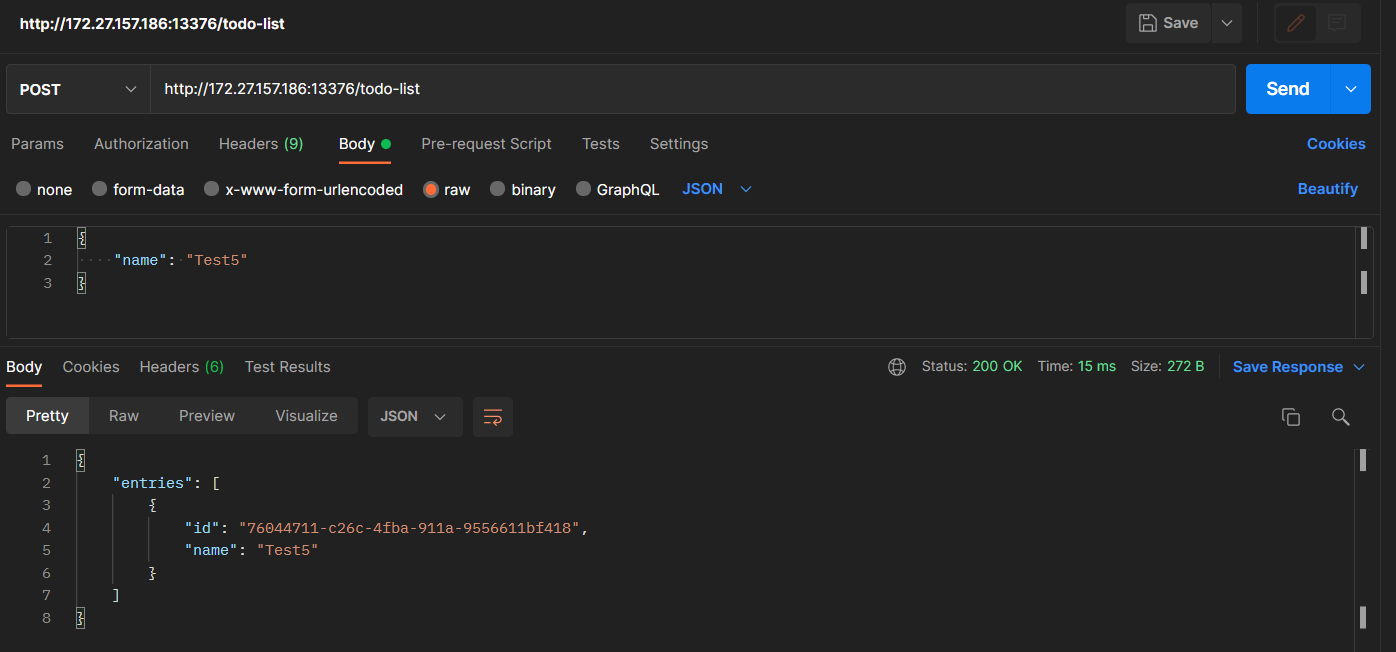
\includegraphics[scale=0.4]{Bilder/api_postman_test_post.png}
        \caption{Teste POST}\label{pic:api_postman_test_post}
    \end{center}
\end{figure}

\begin{figure}[H]
    \begin{center}
        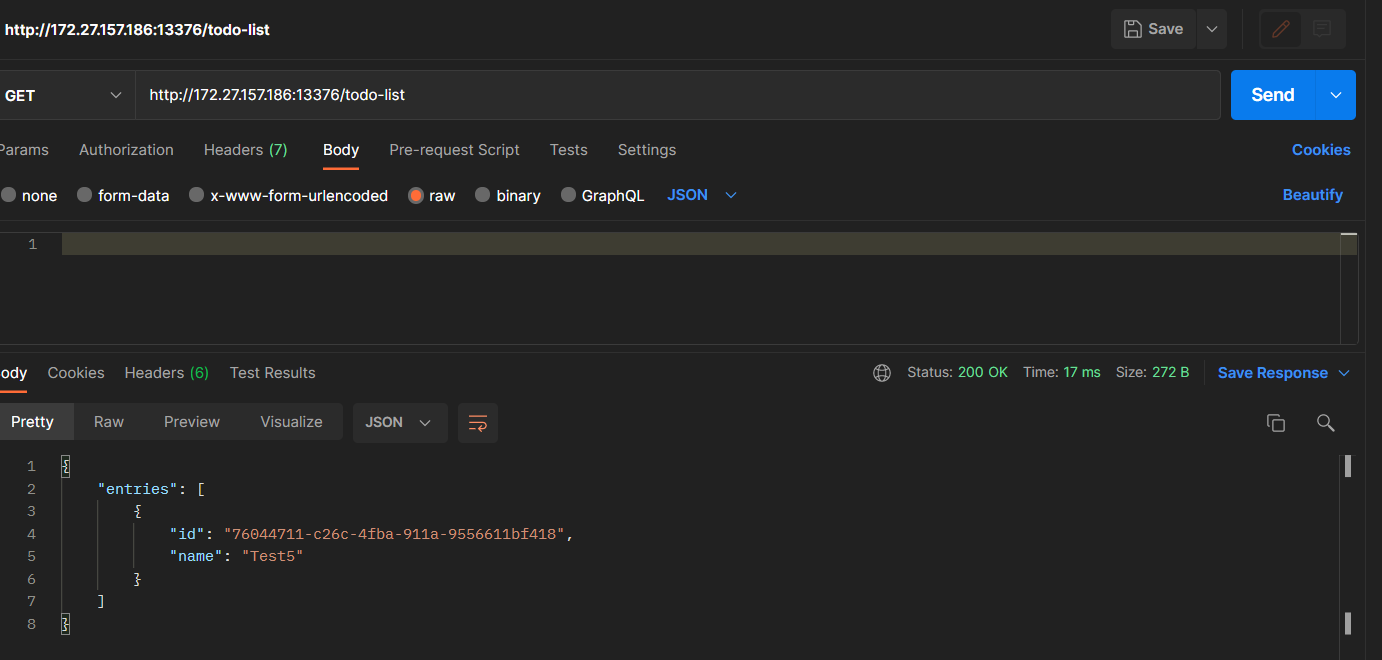
\includegraphics[scale=0.4]{Bilder/api_postman_test_get.png}
        \caption{Teste GET}\label{pic:api_postman_test_get}
    \end{center}
\end{figure}
Es lassen sich neue Todo-Listen anlegen, sowie die existenten Todo-Listen abrufen, die Rest API wurde somit erfolgreich auf dem System installiert.
\\
Nun muss noch sichergestellt werden, dass die API auch nach Neustart des Systems noch erreichbar ist. Dafür muss ein Dienst angelegt werden, der das Skript bei Start
des Systems ausführt. Um den Dienst anzulegen, muss eine \lstinline[basicstyle={\small\ttfamily\color{black}}]|.service| Datei im Systemverzeichnis des Servers angelegt
werden:
\begin{figure}[H]
    \begin{mdframed}[backgroundcolor=bbg]
        \begin{lstlisting}
        <@\textcolor{ssh}{fernzugriff@raspberry}@>:<@\textcolor{path}{$\sim$/todo-api \$}@> cd /lib/systemd/system
        <@\textcolor{ssh}{fernzugriff@raspberry}@>:<@\textcolor{path}{/lib/systemd/system \$}@> sudo nano todoapi.service
        \end{lstlisting}
    \end{mdframed}
    \label{lst:create_service_file}
    % \caption{fernzugriff anlegen}
\end{figure}
In die Datei muss folgender Text eingefügt werden:
\begin{figure}[H]
    \begin{mdframed}[backgroundcolor=bbg]
        \begin{lstlisting}
        <@\textcolor{path}{$\left[\text{Unit}\right]$}@>
        Description=Todo Rest API
        After=multi-user.target
        Conflicts=getty@tty1.service

        <@\textcolor{path}{$\left[\text{Service}\right]$}@>
        Type=simple
        ExecStart=/usr/bin/python3 /home/fernzugriff/todo-api/TodoRestServer/src/App.py
        WorkingDirectory=/home/fernzugriff/todo-api/working
        StandardInput=tty-force

        <@\textcolor{path}{$\left[\text{Install}\right]$}@>
        WantedBy=multi-user.target
        \end{lstlisting}
    \end{mdframed}
    \label{lst:service_file}
    % \caption{fernzugriff anlegen}
\end{figure}
ExecStart ist hier der Befehl, der bei Start des Dienstes ausgeführt wird. Da ein Python Skript ausgeführt werden soll,
Dienste aber nicht mit Umgebungsvariablen arbeiten und somit den Befehl python3 nicht direkt ausführen können, muss hier
der gesamte Pfad zur python3 Datei angegeben werden.
\\
WorkingDirectory gibt den Ordner an, in dem der Befehl ausgeführt werden soll. Schreibt der Befehl zum Beispiel in das Dateisystem,
kann dieser Parameter genutzt werden, um Ablageort des ausgeführten Programms, sowie Speicherort der vom Programm geschriebenen
Dateien voneinander zu trennen.
\\
Da Dienste immer durch den User \glqq root\grqq{} ausgeführt werden, die fehlenden Python-Module aber mit einem anderen
Benutzer heruntergeladen wurden, müssen diese nun auch für den root user heruntergeladen werden. Dafür wird keine Anmeldung
als root benötigt, es reicht, die Installation mit sudo Berechtigungen auszuführen:
\begin{figure}[H]
    \begin{mdframed}[backgroundcolor=bbg]
        \begin{lstlisting}
        <@\textcolor{ssh}{fernzugriff@raspberry}@>:<@\textcolor{path}{$\sim$ \$}@> sudo pip install flask-cors
        \end{lstlisting}
    \end{mdframed}
    \label{lst:install_python_mods_sudo}
    % \caption{fernzugriff anlegen}
\end{figure}
Falls Unklarheit besteht, welche Module dem root User fehlen, kann das Skript der API mit sudo Berechtigungen ausgeführt werden, um zu überprüfen,
ob es möglich ist, dieses mit erhöhten Berechtigungen auszuführen.
\\
Nachdem der Dienst angelegt wurde, muss er nun noch aktiviert und gestartet werden. Zuvor muss aber der Daemon einmal neu geladen werden, damit dieser den neuen Dienst
registriert:
\begin{figure}[H]
    \begin{mdframed}[backgroundcolor=bbg]
        \begin{lstlisting}
        <@\textcolor{ssh}{fernzugriff@raspberry}@>:<@\textcolor{path}{$\sim$ \$}@> sudo systemctl daemon-reload
        <@\textcolor{ssh}{fernzugriff@raspberry}@>:<@\textcolor{path}{$\sim$ \$}@> sudo systemctl enable todoapi.service
        Created symlink /etc/systemd/system/multi-user.target.wants/todoapi.service <@$\rightarrow$@> /lib/systemd/system/todoapi.service.
        <@\textcolor{ssh}{fernzugriff@raspberry}@>:<@\textcolor{path}{$\sim$ \$}@> sudo systemctl start todoapi.service
        \end{lstlisting}
    \end{mdframed}
    \label{lst:enable_service}
    % \caption{fernzugriff anlegen}
\end{figure}
Durch \lstinline[basicstyle={\small\ttfamily\color{black}}]|systemctl enable| wird der Dienst zunächst dem korrekten Userverzeichnis
hinzugefügt, wodurch er in dem entsprechenden Kontext gestartet werden kann. Durch
\lstinline[basicstyle={\small\ttfamily\color{black}}]|systemctl start| wird der Dienst gestartet.
\\
Nun wird das Skript beim Start des Servers direkt hochgefahren.


\section{Nextcloud Container deployen}
Im Folgenden wird beschrieben, wie die Filehosting Lösung Nextcloud als Docker Container deployed wurde.

\subsection{Installation Docker}
Um Nextcloud als Container zu installieren, muss zunächst Docker installiert werden. Da Docker von manchen Linux-Distributionen
ausgeliefert wird, wurden zunächst alle Pakete deinstalliert, die in Konflikt mit den zu installierenden Paketen stehen könnten:
\begin{figure}[H]
    \begin{mdframed}[backgroundcolor=bbg]
        \begin{lstlisting}
        <@\textcolor{ssh}{fernzugriff@raspberry}@>:<@\textcolor{path}{$\sim$ \$}@> for pkg in docker.io docker-doc docker-compose podman-docker containerd runc; do sudo apt-get remove $pkg; done
        \end{lstlisting}
    \end{mdframed}
    \label{lst:uninstall_docker_pkg}
    % \caption{fernzugriff anlegen}
\end{figure}
Der Befehl iteriert über alle Pakete in den angegebenen Repositories und deinstalliert die lokalen Kopien dieser Pakete, sollten
sie installiert sein.
\\
Nachdem die Pakete erfolgreich deinstalliert wurden, musten zunächst Hilfspakete installiert werden, die es ermöglichen, die
notwendigen Voraussetzungen für Docker zu installieren:
\begin{figure}[H]
    \begin{mdframed}[backgroundcolor=bbg]
        \begin{lstlisting}
        <@\textcolor{ssh}{fernzugriff@raspberry}@>:<@\textcolor{path}{$\sim$ \$}@> sudo apt-get install ca-certificates curl gnupg
        \end{lstlisting}
    \end{mdframed}
    \label{lst:install_https_pkgs}
    % \caption{fernzugriff anlegen}
\end{figure}
Anschließend musste der offizielle Docker GPG Key installiert werden, der dazu dient, die Kommunikation zwischen
Docker und dem Docker Repository zu verschlüsseln\footnote{Vgl. Quelle \ref{src:gnupg} in Kapitel\ref{ch:src}}:
\begin{figure}[H]
    \begin{mdframed}[backgroundcolor=bbg]
        \begin{lstlisting}
        <@\textcolor{ssh}{fernzugriff@raspberry}@>:<@\textcolor{path}{$\sim$ \$}@> sudo install -m 0755 -d /etc/apt/keyrings
        <@\textcolor{ssh}{fernzugriff@raspberry}@>:<@\textcolor{path}{$\sim$ \$}@> curl -fsSL https://download.docker.com/linux/ubuntu/gpg | sudo gpg --dearmor -o /etc/apt/keyrings/docker.gpg
        <@\textcolor{ssh}{fernzugriff@raspberry}@>:<@\textcolor{path}{$\sim$ \$}@> sudo chmod a+r /etc/apt/keyrings/docker.gpg
        \end{lstlisting}
    \end{mdframed}
    \label{lst:install_gpg}
    % \caption{fernzugriff anlegen}
\end{figure}
Durch \lstinline[basicstyle={\small\ttfamily\color{black}}]|chmod a+r| wurde des Weiteren jedem User die Berechtigung zur Nutzung des
GPG Keys gegeben.
\\
Nachdem der GPG Key installiert und für jeden Benutzer freigegeben war, konnte das Repository für Docker aufgesetzt werden:
\begin{figure}[H]
    \begin{mdframed}[backgroundcolor=bbg]
        \begin{lstlisting}
        <@\textcolor{ssh}{fernzugriff@raspberry}@>:<@\textcolor{path}{$\sim$ \$}@> echo \
        "deb [arch="$(dpkg --print-architecture)" signed-by=/etc/apt/keyrings/docker.gpg] https://download.docker.com/linux/ubuntu \
        "$(. /etc/os-release && echo "$VERSION_CODENAME")" stable" | \
        sudo tee /etc/apt/sources.list.d/docker.list > /dev/null
        \end{lstlisting}
    \end{mdframed}
    \label{lst:setup_docker_repo}
    % \caption{fernzugriff anlegen}
\end{figure}
Final konnte nun Docker installiert werden:
\begin{figure}[H]
    \begin{mdframed}[backgroundcolor=bbg]
        \begin{lstlisting}
        <@\textcolor{ssh}{fernzugriff@raspberry}@>:<@\textcolor{path}{$\sim$ \$}@> sudo apt-get install docker-ce docker-ce-cli containerd.io docker-buildx-plugin docker-compose-plugin
        \end{lstlisting}
    \end{mdframed}
    \label{lst:install_docker}
    % \caption{fernzugriff anlegen}
\end{figure}
Um zu überprüfen, ob die Installation erfolgreich war, konnte nun ein einfaches Docker Image gestartet werden:
\begin{figure}[H]
    \begin{mdframed}[backgroundcolor=bbg]
        \begin{lstlisting}
        <@\textcolor{ssh}{fernzugriff@raspberry}@>:<@\textcolor{path}{$\sim$ \$}@> sudo docker run hello-world
        \end{lstlisting}
    \end{mdframed}
    \label{lst:setup_docker_repo}
    % \caption{fernzugriff anlegen}
\end{figure}


\subsection{Einrichtung Nextcloud als Docker Container}
Da Docker automatisch alle Images, die nicht bereits installiert sind, bei Ausführung aus der Image Registry herunterlädt und installiert, muss nur der Befehl ausgeführt werden,
um das Nextcloud Image zu starten. Da Docker Container nicht persistent sind, muss allerdings noch ein Dateiverzeichnis angegeben werden, in dem die Dateien gespeichert werden:
\begin{figure}[H]
    \begin{mdframed}[backgroundcolor=bbg]
        \begin{lstlisting}
        <@\textcolor{ssh}{fernzugriff@raspberry}@>:<@\textcolor{path}{$\sim$ \$}@> sudo mkdir "/var/nc-files"
        <@\textcolor{ssh}{fernzugriff@raspberry}@>:<@\textcolor{path}{$\sim$ \$}@> sudo docker run -v "/var/nc-files" nextcloud
        \end{lstlisting}
    \end{mdframed}
    \label{lst:folder_for_nextcloud}
    % \caption{fernzugriff anlegen}
\end{figure}
Nachdem der Befehl ausgeführt wurde, wird zunächst das Image, falls es noch nicht lokal installiert ist, heruntergeladen. Anschließend wird das Image als Container ausgeführt, wobei
der Pfad, der hinter dem \lstinline[basicstyle={\small\ttfamily\color{black}}]|-v| Parameter angegeben ist, als Volume für den Container dient. Sobald der Container als Dienst
installiert wurde, wurde den einzelnen Komponenten der Nextcloud jeweils eine eigene Volume zugewiesen, dies war zunächst nur ein Test.
\\
Des Weiteren sollte die Weboberfläche der Nextcloud von anderen Hosts erreichbar sein. Um dies zu realisieren, musste zunächst ein weiterer Port in der Firewall freigegeben
werden. Die Wahl ist auf den Port 8080 gefallen, hier kann aber ein beliebiger freier Port genutzt werden:
\begin{figure}[H]
    \begin{mdframed}[backgroundcolor=bbg]
        \begin{lstlisting}
        <@\textcolor{ssh}{fernzugriff@raspberry}@>:<@\textcolor{path}{$\sim$ \$}@> sudo ufw allow 8080
        Rules updated
        Rules updated (v6)
        \end{lstlisting}
    \end{mdframed}
    \label{lst:port_nextcloud}
    % \caption{fernzugriff anlegen}
\end{figure}
Außerdem musste der Container mit dem entsprechenden Port gestartet werden:
\begin{figure}[H]
    \begin{mdframed}[backgroundcolor=bbg]
        \begin{lstlisting}
        <@\textcolor{ssh}{fernzugriff@raspberry}@>:<@\textcolor{path}{$\sim$ \$}@> sudo docker run -p 8080:80 -v "/var/nc-files" nextcloud
        \end{lstlisting}
    \end{mdframed}
    \label{lst:port_nextcloud}
    % \caption{fernzugriff anlegen}
\end{figure}
Der Parameter \lstinline[basicstyle={\small\ttfamily\color{black}}]|-p 8080:80| gibt hierbei an, dass HTTP Requests auf dem Port 8080 die Weboberfläche der Nextcloud aufrufen
sollen. Nun war die Weboberfläche erreichbar:
\begin{figure}[H]
    \begin{center}
        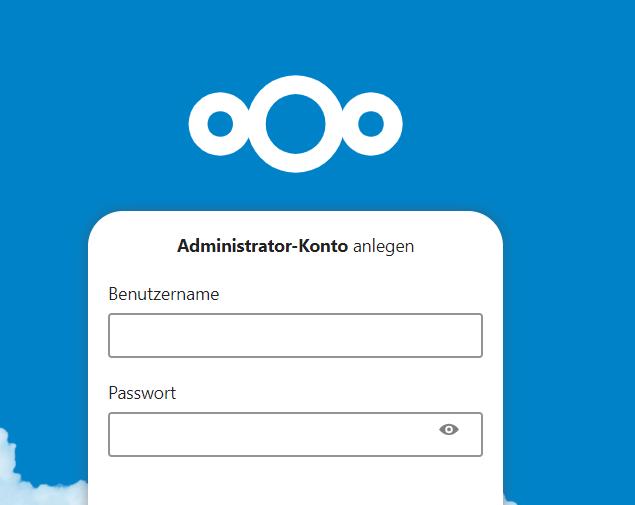
\includegraphics[scale=0.5]{Bilder/nextcloud_web.png}
        \caption{Nextcloud Weboberfläche}
    \end{center}
\end{figure}
Bevor die Konfiguration der Nextcloud fortgesetzt wurde, wurde ein Dienst angelegt, damit der Container beim Start des Systems verfügbar war. Da die Konfiguration
identisch zu der aus Kapitel \ref{ch:api_os} abläuft, wird das Vorgehen hier nicht weiter erläutert:
\begin{figure}[H]
    \begin{mdframed}[backgroundcolor=bbg]
        \begin{lstlisting}
        <@\textcolor{ssh}{fernzugriff@raspberry}@>:<@\textcolor{path}{$\sim$ \$}@> cd /lib/systemd/system
        <@\textcolor{ssh}{fernzugriff@raspberry}@>:<@\textcolor{path}{/lib/systemd/system \$}@> sudo nano nextcloud.service
        \end{lstlisting}
    \end{mdframed}
    \label{lst:create_service_file_nextcloud}
    % \caption{fernzugriff anlegen}
\end{figure}

\begin{figure}[H]
    \begin{mdframed}[backgroundcolor=bbg]
        \begin{lstlisting}
        <@\textcolor{path}{$\left[\text{Unit}\right]$}@>
        Description=Nextcloud Service
        After=multi-user.target
        Conflicts=getty@tty7.service

        <@\textcolor{path}{$\left[\text{Service}\right]$}@>
        Type=simple
        ExecStart=/usr/bin/docker run -p 8080:80 \
        -v db:/var/lib/sqlite \
        -v data:/var/www/html/data \
        -v nextcloud:/var/www/html \
        -v custom_apps:/var/www/html/custom_apps \
        -v config:/var/www/html/config \
        -v themes:/var/www/html/themes \
        nextcloud
        StandardInput=tty-force

        <@\textcolor{path}{$\left[\text{Install}\right]$}@>
        WantedBy=multi-user.target
        \end{lstlisting}
    \end{mdframed}
    \label{lst:service_file}
    % \caption{fernzugriff anlegen}
\end{figure}

\begin{figure}[H]
    \begin{mdframed}[backgroundcolor=bbg]
        \begin{lstlisting}
        <@\textcolor{ssh}{fernzugriff@raspberry}@>:<@\textcolor{path}{$\sim$ \$}@> sudo systemctl daemon-reload
        <@\textcolor{ssh}{fernzugriff@raspberry}@>:<@\textcolor{path}{$\sim$ \$}@> sudo systemctl enable nextcloud.service
        Created symlink /etc/systemd/system/multi-user.target.wants/todoapi.service <@$\rightarrow$@> /lib/systemd/system/nextcloud.service.
        <@\textcolor{ssh}{fernzugriff@raspberry}@>:<@\textcolor{path}{$\sim$ \$}@> sudo systemctl start nextcloud.service
        \end{lstlisting}
    \end{mdframed}
    \label{lst:enable_service}
    % \caption{fernzugriff anlegen}
\end{figure}
Um zu überprüfen, ob der neue Dienst aktiv ist, wurden zuletzt noch alle aktiven Docker Images angezeigt:
\begin{figure}[H]
    \begin{mdframed}[backgroundcolor=bbg]
        \begin{lstlisting}
        <@\textcolor{ssh}{fernzugriff@raspberry}@>:<@\textcolor{path}{$\sim$ \$}@> sudo docker ps
        CONTAINER IDs       Image       COMMAND                     CREATED         <@\textcolor{path}{\#...}@>
        5f3bc0925087        nextcloud   "/entrypoint.sh apac..."    50 seconds ago  <@\textcolor{path}{\#...}@>
        \end{lstlisting}
    \end{mdframed}
    \label{lst:enable_service}
    % \caption{fernzugriff anlegen}
\end{figure}
Nextcloud war somit erfolgreich installiert, die Daten persistiert und der Container wurde bei Start des Systems hochgefahren.
\\
Nun konnte die Nextcloud final konfiguriert werden. Beim Initialen Aufruf der Weboberfläche erwartet Nextcloud die Anlage eines administrativen Benutzers. Hier wurden
ein Nutzer und ein Passwort hinterlegt.
\\
Nextcloud war somit fertig installiert und eingerichtet:
\begin{figure}[H]
    \begin{center}
        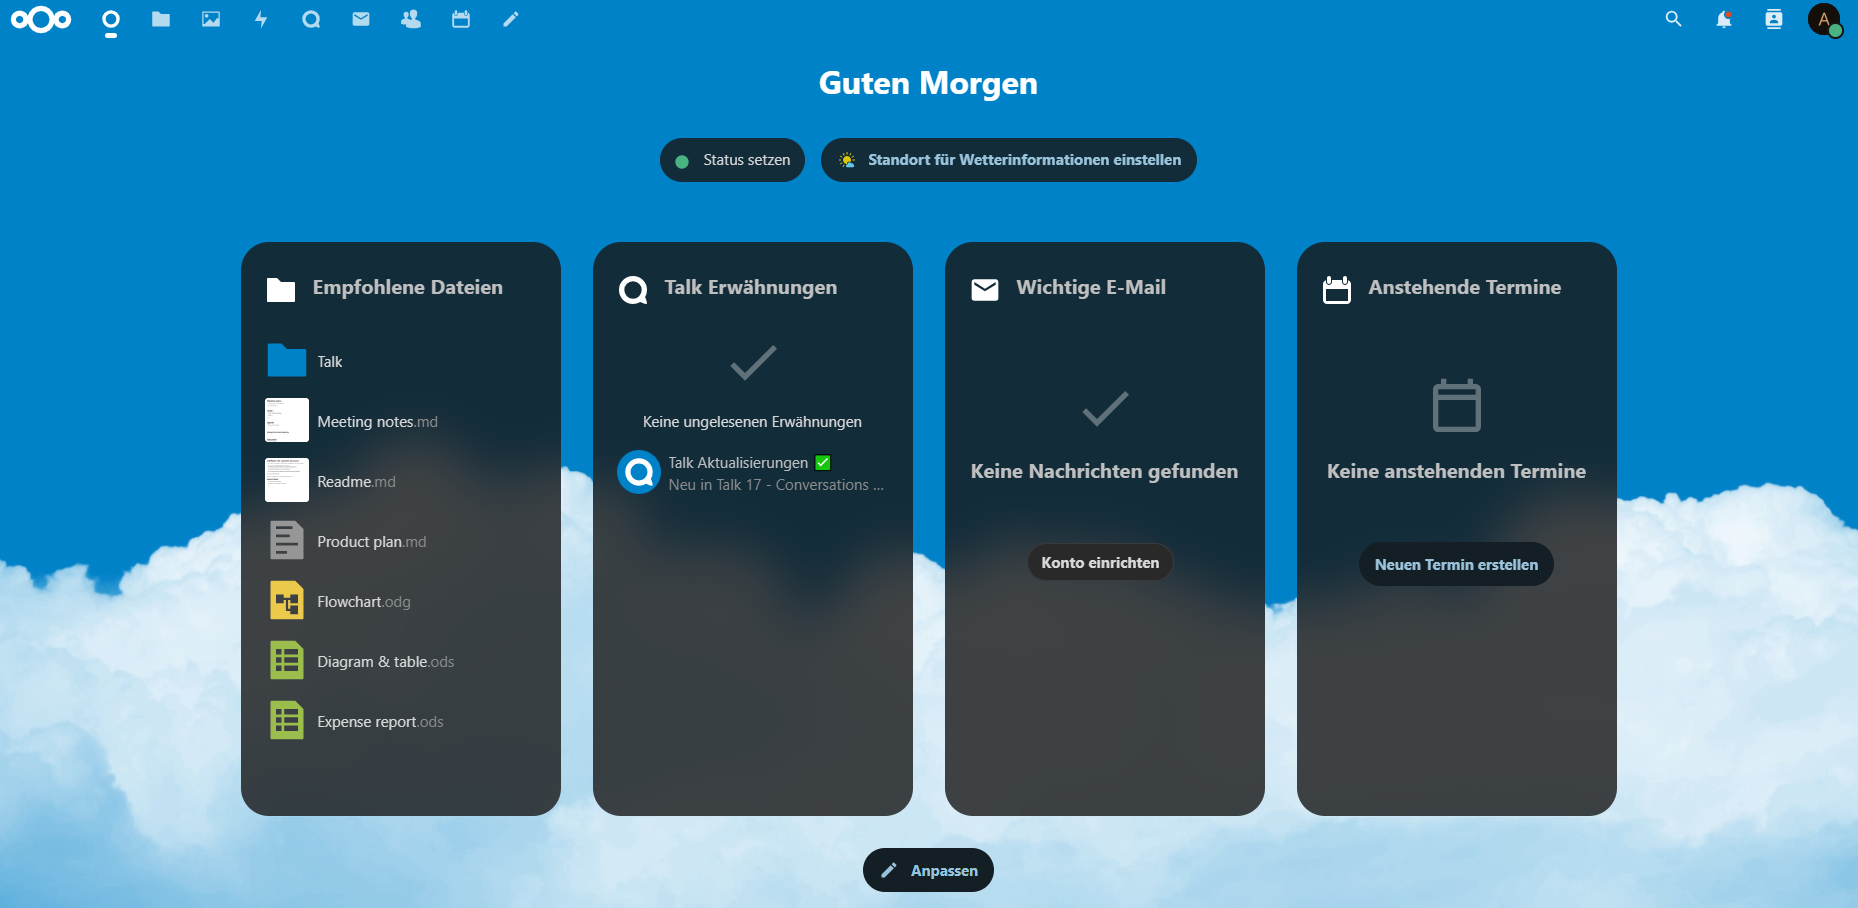
\includegraphics[scale=0.2]{Bilder/nextcloud_web_app.png}
        \caption{Nextcloud Web Oberfläche}
    \end{center}
\end{figure}



\newpage
\section{Anlagen}
\subsection{Quellen}\label{ch:src}
\begin{enumerate}
    \item Ubuntu Wiki: UncomplicatedFirewall. 2022 - Online unter: \newline\url{https://wiki.ubuntu.com/UncomplicatedFirewall} $\left[\text{11.06.2023}\right]$\label{src:ufw}
    \item GnuPG: The GNU Privacy Guard. Online unter: \newline\url{https://gnupg.org/} $\left[\text{22.06.2023}\right]$\label{src:gnupg}
\end{enumerate}
\begin{small}

\end{small}
\end{document}